\section{Results}\label{sec:results}
% todo talk also about the training problems, the loss function that stops reducing for example.
% %**************************************************************

\subsection{Full sequence prediction}\label{subsec:full-sequence-prediction}
With different models a variety of results are achieved, but the most important result is that an important baseline for the future development of this kind of systems has been settled down.
After a few trials with few models, which produced some circular trajectories, with the encoder-only version of transformer, and feeding the \textit{sequence 3} of Kitti (for more details \S~\ref{sec:kitti}) where the first image is considered as origin, we showed that the model is able to learn a single sequence in over-fitting, but fails when trying to over-fit a more complex sequence.

The encoder-decoder version achieved the same results as the previous version, but the model was able to learn also the \textit{sequence 7} of Kitti, but it fails when trained with both \textit{sequence 3} and \textit{sequence 7}.
\begin{figure}[H]
    \centering
    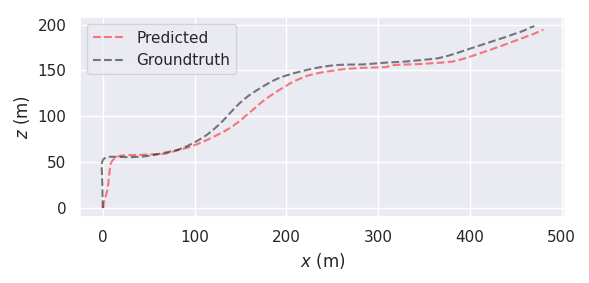
\includegraphics[width=0.8\textwidth]{images/6_1_well_predicted_seq_3}
    \caption{Good prediction sequence 3}\label{fig:well-predicted-seq-3}
\end{figure}
\begin{figure}[H]
    \centering
    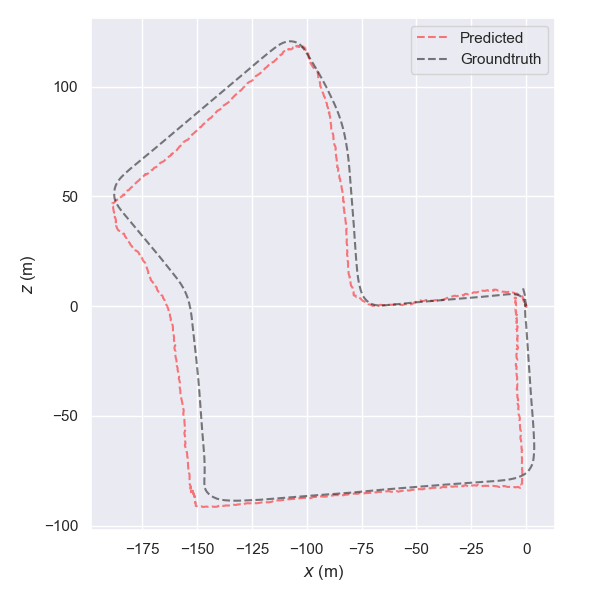
\includegraphics[width=0.8\textwidth]{images/6_1_well_predicted_seq_7}
    \caption{Good prediction sequence 7}\label{fig:well-predicted-seq-7}
\end{figure}
% %**************************************************************

\subsection{Autoregressive models}\label{subsec:autoregressive-model}
We implemented only the encoder-decoder version of the transformer in the autoregressive way, and most of the time the prediction of the network during the training on seq 3 is just a straight line.
So the model is \textbf{not} able to predict the simplest sequence in over-fitting.
The model could not predict any reasonable trajectory, predicting only a linear trajectory as the follow:
\begin{figure}[H]
    \centering
    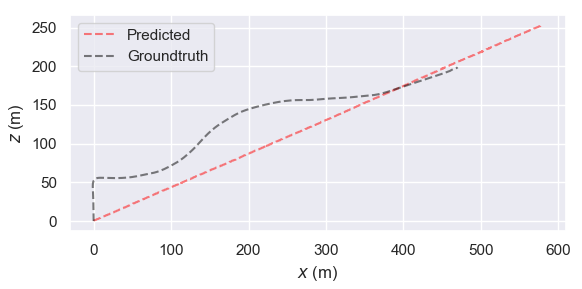
\includegraphics[width=0.8\textwidth]{images/6_1_autoregressive_prediction}
    \caption{Bad prediction sequence 3 of autoregressive model}\label{fig:autoregressive-seq-3}
\end{figure}
Although the model has been trained for more than two hundred epochs, the network cannot understand the goal, and this maybe is due to the loss function.